\chapter{Abordagem}
\label{sec:abordagem}

Este capítulo tem como principal objectivo descrever a metodologia adotada e ainda apresentar o planeamento do projeto tal como os desvios relativamente ao mesmo. Por fim será apresentada uma análise dos riscos associados ao projeto, que poderão ter um impacto negativo no plano de desenvolvimento. Este conjunto de passos foca-se em atingir um produto final bem estruturado e funcional, utilizando boas práticas de desenvolvimento de software.


\section{Metodologia}
\label{metodologia}

A metodologia de desenvolvimento do projeto adoptada baseada-se fortemente em SCRUM\cite{scrum}, que será descrita (i. e. os aspectos mais importantes) nesta secção. Esta é a metodologia utilizada pela 10.digital e tendo em conta que esta metodologia ágil se encaixa perfeitamente nas necessidades do projeto, estes foram os fatores decisivos para a escolha da mesma. 

Líder em desenvolvimento ágil, o SCRUM, é uma metodologia apontada para projetos com foco em trazer valor ao cliente de forma incremental, através de iterações de curta duração, chamadas \textit{Sprints}. Esta metodologia possibilita também a abordagem de problemas complexos de forma produtiva, priorizar tarefas durante a fase de desenvolvimento e ainda facilita a inclusão de novas funcionalidades sempre que necessário. Desta forma o SCRUM proporciona uma gestão flexível do projeto e permite realizar pequenas alterações no planeamento, sem necessidade de interromper o desenvolvimento.

\subsection{Intervenientes}

Um aspecto determinante para o sucesso do SCRUM é o trabalho em equipa. Tipicamente nesta metodologia existem três papéis pré-definidos: \textit{Product Owner}, \textit{Scrum Master} e \textit{Scrum Team}.

O \textbf{\textit{Product Owner}} representa o cliente e é responsável por transmitir a visão do produto, ou por outras palavras, é responsável por maximizar o valor do produto e o trabalho da equipa de desenvolvimento (i. e. \textit{Scrum Master}). É responsável por organizar e priorizar as tarefas no \textit{product backlog}.

O \textbf{\textit{Scrum Master}} tem um papel fundamental no desempenho da \textit{Scrum Team}. É responsável por garantir o cumprimento das práticas do SCRUM, ajudar e orientar a \textit{Scrum Team} especialmente nas dificuldades que vão surgindo ao longo do projeto e, de forma gradual (i. e. respeitando as \textit{Sprints}), apresentar o trabalho realizado ao \textit{Product Owner}.

A \textbf{\textit{Scrum Team}} representa os elementos que constituem a equipa de desenvolvimento que com a orientação do \textit{Scrum Master}, monitorizam o trabalho que vai sendo feito e assim conseguir cumprir com as \textit{sprints backlog}. A \textit{Scrum Team} deve ser autónoma e organizada. 

\subsection{Processo}

O Desenvolvimento começa assim que o \textit{product backlog} estiver concluído e detalhado pelo \textit{Product Owner}. O \textit{product backlog} representa a lista de requisitos necessários para atingir o produto final. 

Depois de definido o \textit{product backlog}, o \textit{Scrum Master}, juntamente com a \textit{Scrum Team} reúnem e definem o tempo para cada \textit{Sprint}. Tipicamente as \textit{Sprints} tem duração entre 1 a 4 semanas e no final das mesmas é apresentado o trabalho realizado pela \textit{Scrum Team}. No início de cada \textit{Sprint} é criada a \textit{Sprint Backlog}, onde é estipulado o conjunto de funcionalidades/tarefas a realizar durante a \textit{Sprint}. Na 10.digital a variável da velocidade não é implementada na \textit{Sprint Backlog}.

No início de cada dia é realizada a \textit{Daily Scrum}, uma reunião que tem uma duração de 15$\pm$5 minutos, onde, de forma informal, são discutidas as tarefas que devem ser implementadas nesse dia, o ponto de situação do projeto relativo ao dia anterior e caso haja algum impasse ou dificuldade na realização de alguma tarefa, imediatamente após a reunião (i. e. assim que possível) tenta-se arranjar uma solução para o mesmo. 

No final de cada \textit{Sprint} há uma reunião (\textit{Sprint Review}) para verificar as tarefas que foram realizadas. Durante a reunião a \textit{Scrum Team} apresenta as novas funcionalidades implementadas para os restantes participantes que podem ser \textit{Product Owner}, \textit{Scrum Master}, clientes e outros colegas de trabalho. 

A Figura \ref{fig:scrum} sumariza todo o processo descrito anteriormente.



\begin{figure}[ht!]
	\begin{center}
		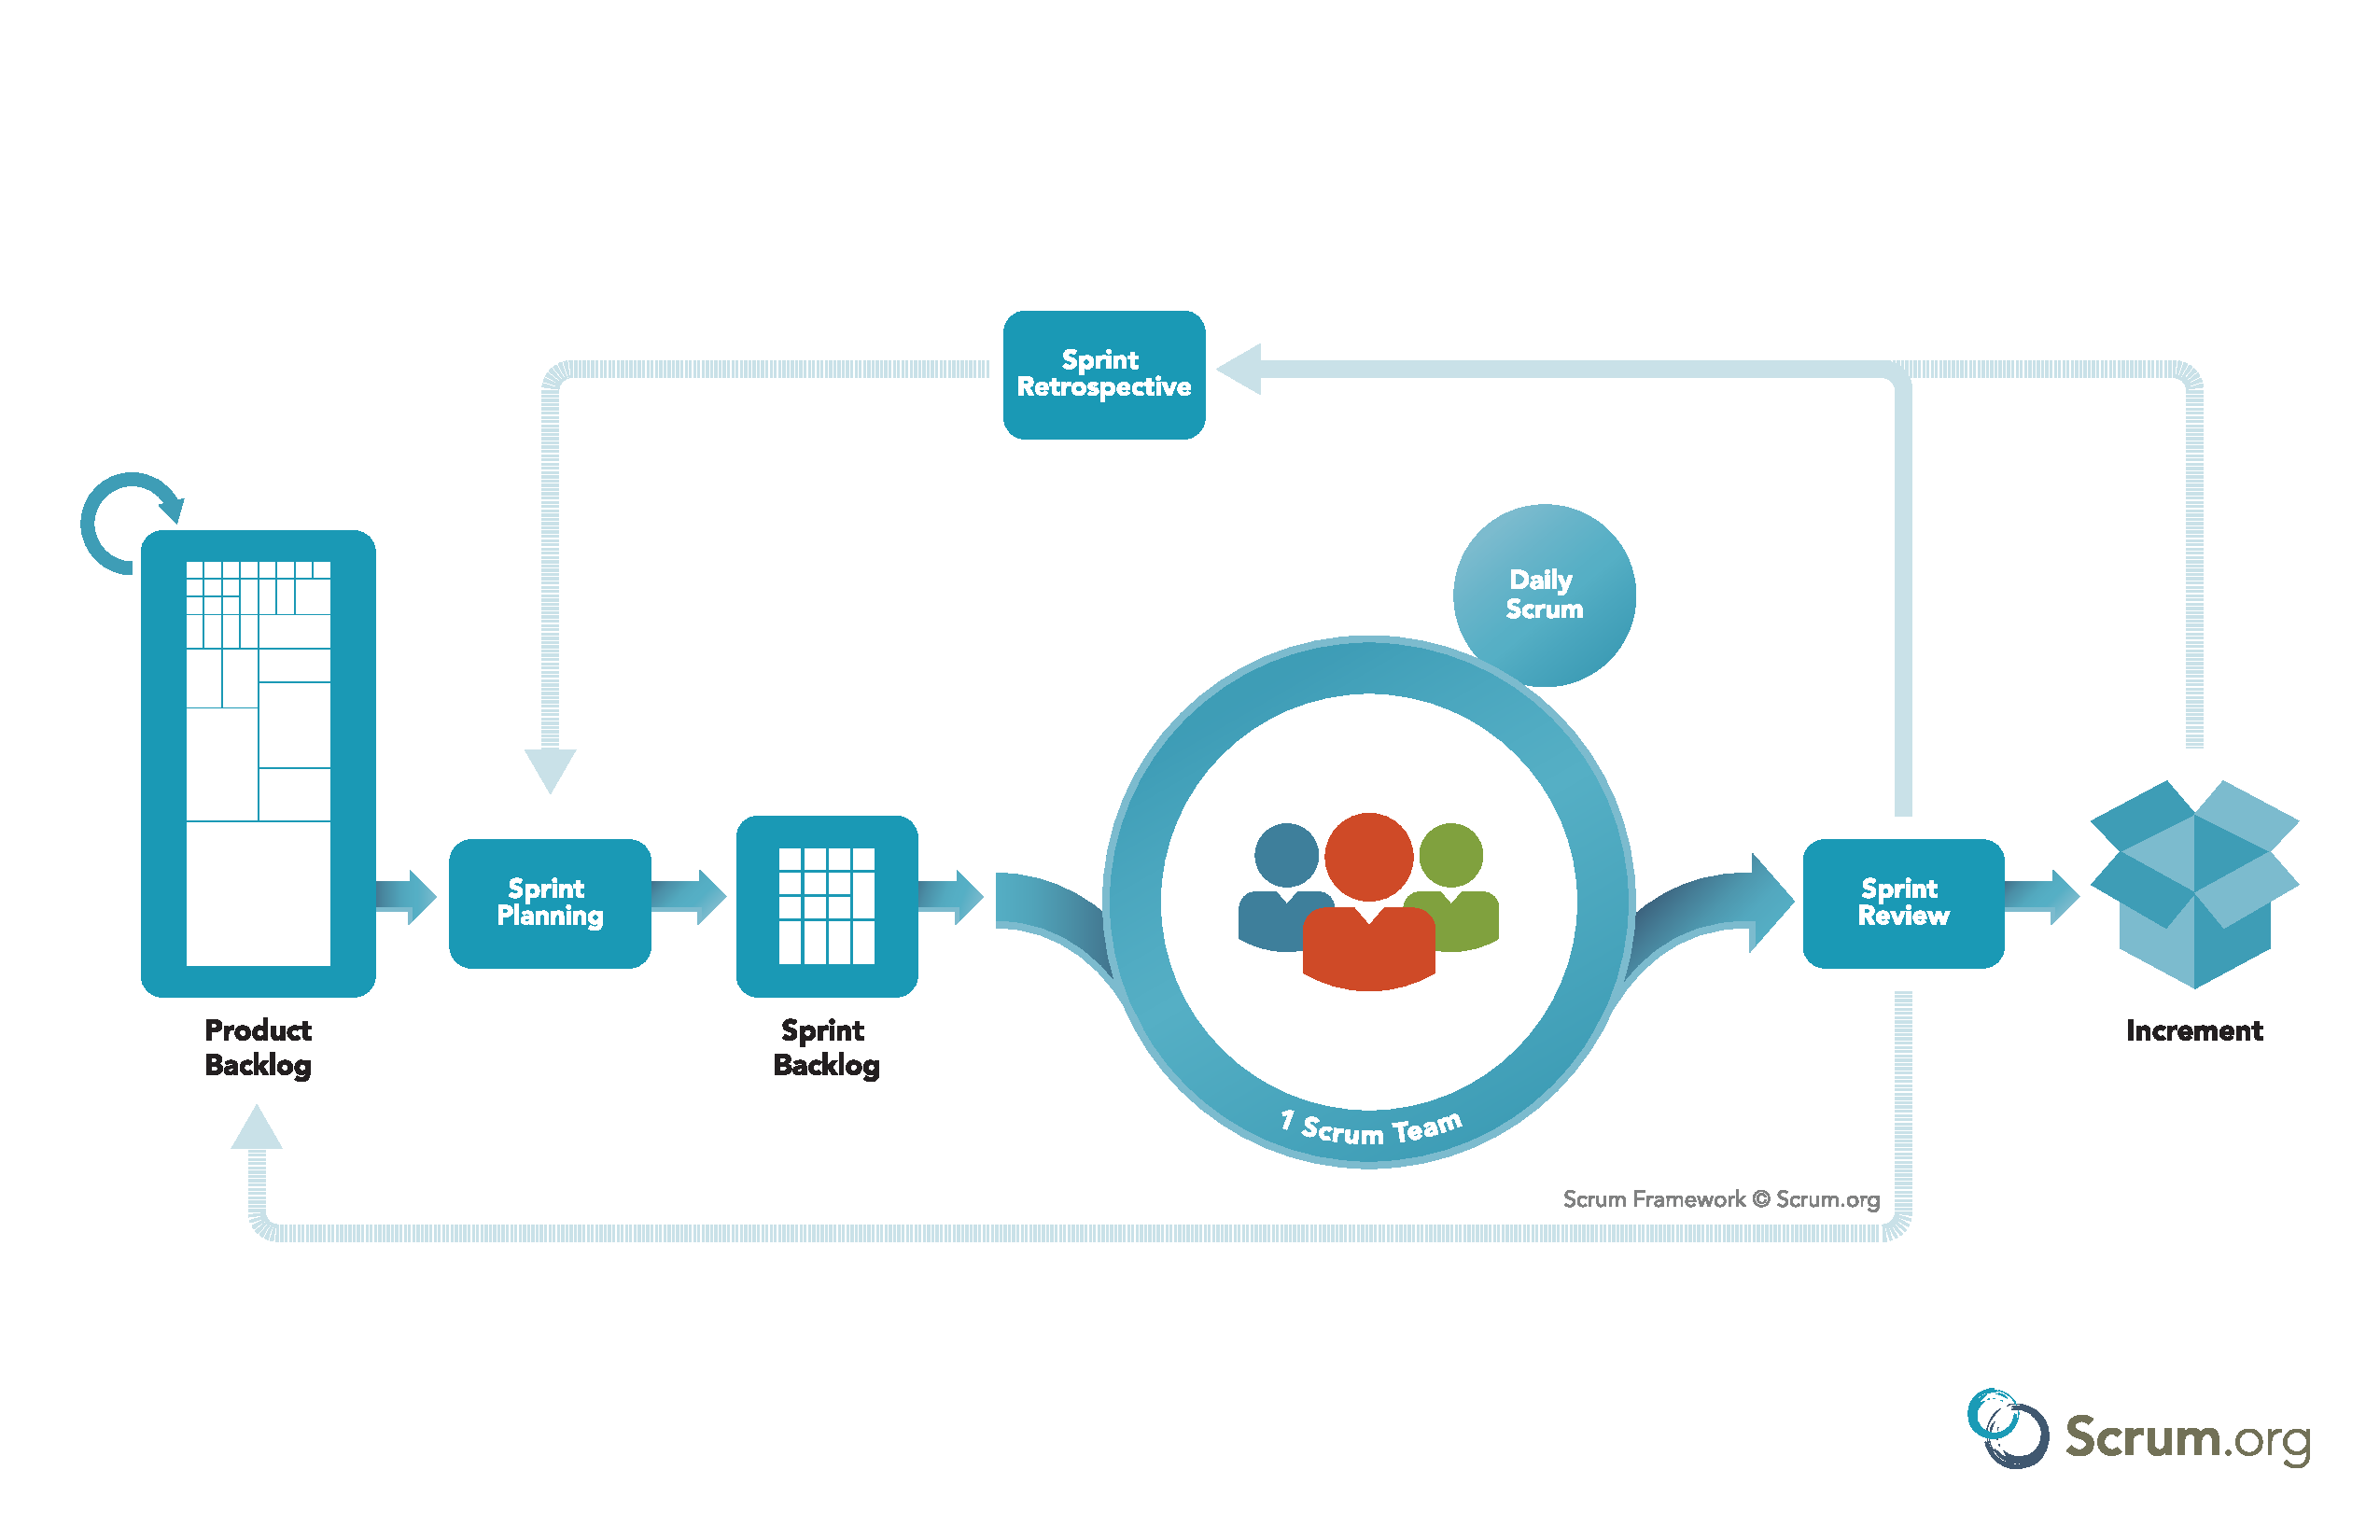
\includegraphics[width=1\textwidth]{img/scrum.pdf}
		\caption{Scrum Framework\cite{scrumimg}}
		\label{fig:scrum}
	\end{center}
\end{figure}

\newpage

\section{Planeamento}
\label{planeamento}

Nesta secção será apresentado o plano de estágio do primeiro e segundo semestre, através de diagramas de Gantt.  De seguida será exposto o desvio temporal em relação ao planeado e por fim serão brevemente detalhados os artefactos (i. e. \textit{Sprint Backlog}) da metodologia SCRUM.

Como foi referido no Capítulo \ref{sec:introducao}, este documento expõe o trabalho realizado neste projeto durante o ano lectivo, por isso, apenas será exposto o desenvolvimento do \textit{back-end} da plataforma de inbound marketing. Dito isto, a equipa de desenvolvimento será composta por múltiplas pessoas sendo que cada um terá a sua função distinta.
No seguimento do ponto anterior, os cargos de cada interveniente no projeto são:
\begin{itemize}
	\item[--] \textbf{\textit{Product Owner}}: Eng. Pedro Beck (\acrfull{cto})
	\item[--] \textbf{\textit{Scrum Master}}: Mário Melo (Coordenador de Projetos)
	\item[--] \textbf{\textit{Scrum Team}}: 
	\subitem  \textit{Front-End Developer} - Ernest Cruz
	\subitem  \textit{Front-End e Back-End Developer} - Bruno Grifo
	\subitem  \textit{Senior Developer \acrshort{tcg}} - Eng. Pedro Beck
\end{itemize}

É ainda de referir que, no primeiro semestre, o Mestre João Oliveira realizou o papel de co-orientador na empresa e teve um impacto importante na orientação do projeto de tese. 

\subsection{Primeiro Semestre}

Nesta secção está detalhado o plano das tarefas associados ao primeiro semestre seguido das respectivas \textit{sprints}.

\begin{figure}[ht!]
	\begin{center}
		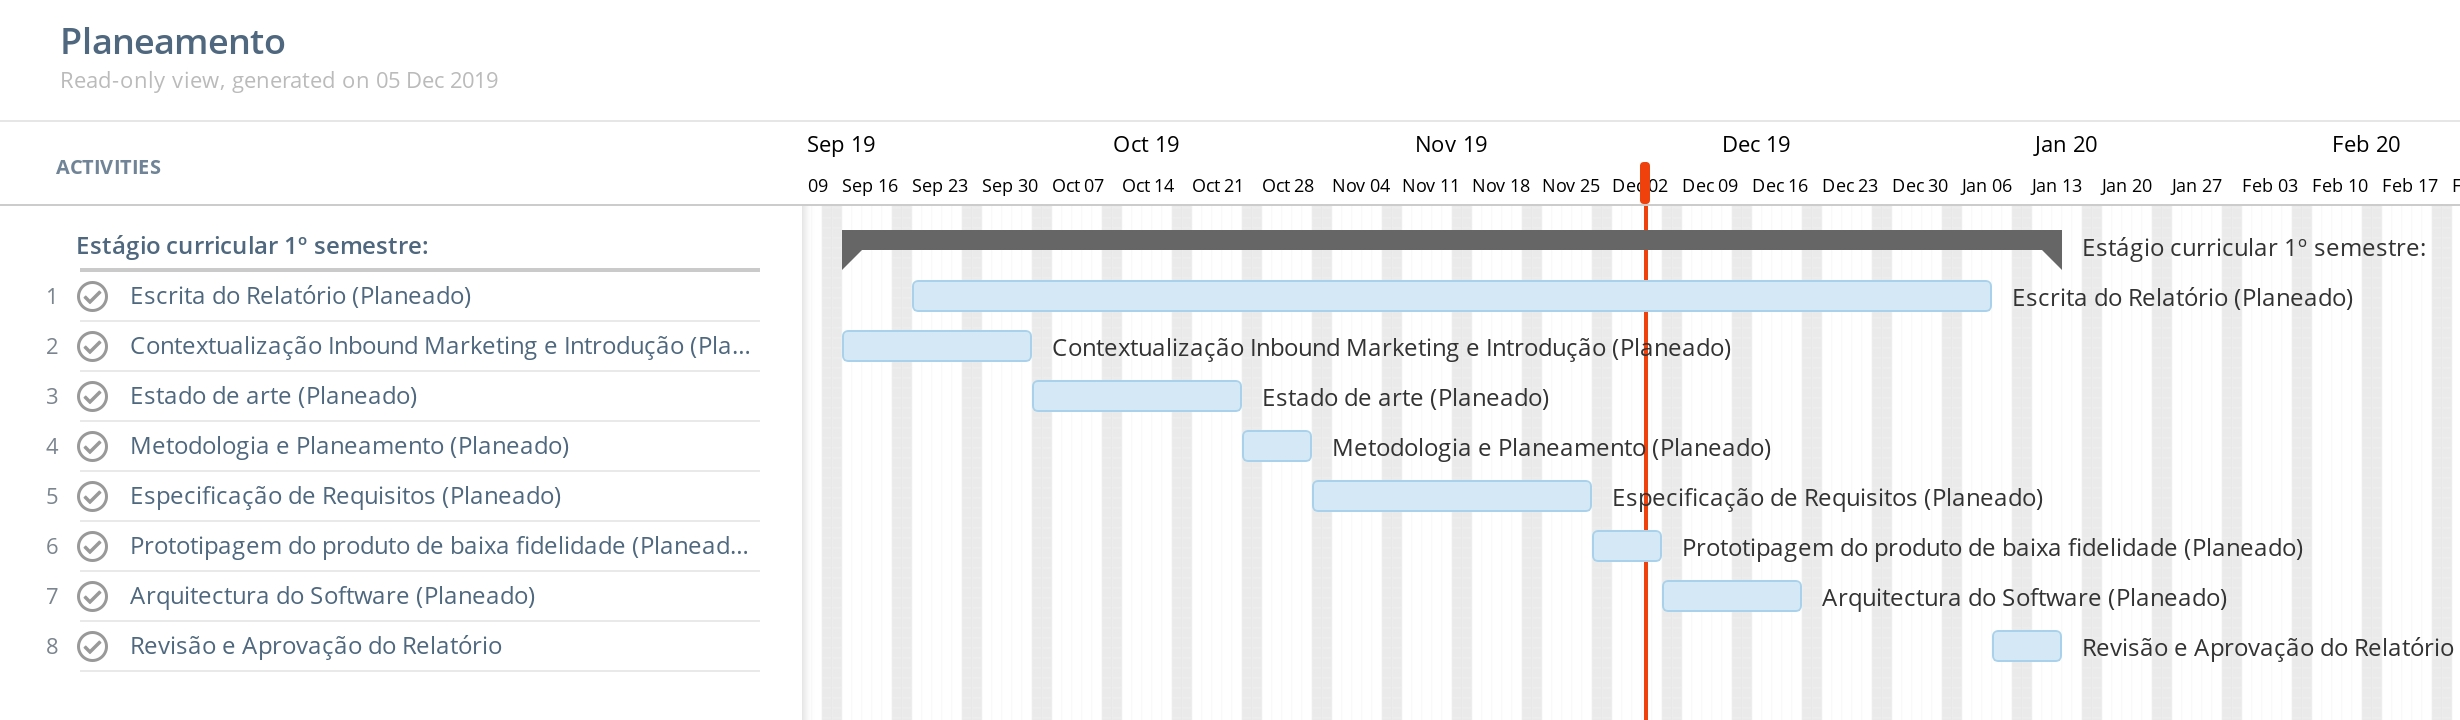
\includegraphics[width=1\textwidth]{img/gantt/semestre1.jpeg}
		\caption{Diagrama de Gantt - Planeamento do 1º semestre}
		\label{fig:gantt1}
	\end{center}
\end{figure}

Representado na Figura \ref{fig:gantt1} apresenta-se o plano de estágio relativo ao primeiro semestre. A redação do relatório intermédio foi dividido nas seguintes 6 tarefas principais:
\begin{itemize}
	\item \textbf{Contextualização de Inbound Marketing e Introdução}: Tendo em conta a área onde o projeto se insere, foi realizado um estudo sobre inbound marketing de modo a  facilitar a compreensão e contextualização das diversas estratégias de inbound. No final da tarefa foi realizada uma apresentação sobre este tema e avaliada pelo co-orientador da empresa, para garantir o nível de conhecimento pretendido. Este estudo foi crucial para desenhar o modelo de negócio do projeto.
	\item \textbf{Estado de Arte}: Nesta tarefa foi feito o levantamento do estado de arte. Foram analisadas várias aplicações/plataformas concorrentes ou com funcionalidades semelhantes para ganhar um melhor conhecimento sobre o mercado.
	\item \textbf{Metodologia e Planeamento}: Foi realizado um estudo interno para perceber ao detalhe como foi adoptada a metodologia SCRUM na empresa e foi também feita a análise de riscos associados ao projeto.
	\item \textbf{Especificação de Requisitos}: Esta tarefa iniciou-se com a elaboração de alguns protótipos de baixa fidelidade e um conjunto de requisitos funcionais. Após a reunião com o cliente, com base no trabalho realizado anteriormente, foram feitos os devidos ajustes e levantados os restantes requisitos. Foram assim documentados os requisitos não funcionais, funcionais e respetivos casos de uso e ainda as restrições técnicas e de negócios.
	\item \textbf{Prototipagem de produto de baixa fidelidade}: Foi criado um conjunto de protótipos, que representam todas as funcionalidades principais da plataforma, e que de igual forma satisfazem o caso de uso correspondente.
	\item \textbf{Arquitetura de Software}: Nesta tarefa foi projetada a arquitetura a desenvolver no âmbito do estágio.
\end{itemize}

Neste projeto cada \textit{sprint} tem duração de duas semanas e a \textit{sprint meeting} é feita no último dia. Em cada\textit{ sprint meeting }está presente a equipa de desenvolvimento (\textit{scrum team}), os orientadores (\textit{product owner}) e, sempre que possível, o tutor. Cada estagiário apresenta o que fez durante o \textit{sprint}, executa a \textit{demo} das funcionalidades implementadas e partilha as dificuldades encontradas durante o \textit{sprint }com os restantes. Os orientadores dão \textit{feedback}, tanto do resultado geral do \textit{sprint}, como de cada funcionalidade (\textit{user story}) implementada.


Neste semestre cada \textit{sprint} tem a duração de 2 semanas e no final da mesma é feita uma reunião de ponto (i. e. \textit{Daily Scrum}), onde estão presentes o \textit{Product Owner}, \textit{Scrum Master}, clientes e outros colegas de trabalho que queiram participar. Nesta primeira fase, no total foram realizadas 7 \textit{Sprints}:

\begin{itemize}
	\item \textbf{\textit{Sprint} \#1}
		\subitem \textbf{Data Início}: 16/09/2019
		\subitem \textbf{Data Fim}: 27/09/2019
		\subitem \textbf{Descrição}: Estudo sobre Inbound Marketing.
	\item \textbf{\textit{Sprint} \#2}
		\subitem \textbf{Data Início}: 28/09/2019
		\subitem \textbf{Data Fim}: 11/10/2019
		\subitem \textbf{Descrição}: Escrita do Capítulo \ref{sec:introducao} e início do estudo sobre aplicações/plataformas concorrentes.
	\item \textbf{\textit{Sprint} \#3}
		\subitem \textbf{Data Início}: 12/10/2019
		\subitem \textbf{Data Fim}: 25/10/2019
		\subitem \textbf{Descrição}: Conclusão do estudo de mercado e escrita do Capítulo \ref{sec:estado-arte}.
	\item \textbf{\textit{Sprint} \#4}
		\subitem \textbf{Data Início}: 26/10/2019
		\subitem \textbf{Data Fim}: 08/11/2019
		\subitem \textbf{Descrição}: Escrita do Capítulo \ref{sec:abordagem} e reunião com o cliente para levantamento de requisitos.
	\item \textbf{\textit{Sprint} \#5}
		\subitem \textbf{Data Início}: 09/11/2019
		\subitem \textbf{Data Fim}: 22/11/2019
		\subitem \textbf{Descrição}: Escrita do Capítulo \ref{sec:requisitos}.
	\item \textbf{\textit{Sprint} \#6}
		\subitem \textbf{Data Início}: 23/11/2019
		\subitem \textbf{Data Fim}: 06/12/2019
		\subitem \textbf{Descrição}:  Escrita dos casos de Uso no Anexo \ref{a:cu} e prototipagem do produto de baixa fidelidade no Anexo \ref{a:prototipos}.
	\item \textbf{\textit{Sprint} \#7}
		\subitem \textbf{Data Início}: 06/11/2019
		\subitem \textbf{Data Fim}: 20/12/2019
		\subitem \textbf{Descrição}: Projeção da arquitectura e escrita do Capítulo \ref{sec:arquitetura}
\end{itemize}


\subsection{Segundo Semestre}
\label{sec:sprints}

À semelhança do primeiro semestre, o desenvolvimento do projecto foi dividido em sprints. Como foi referido anteriormente as sprints têm uma duração de 2 semanas e foram planeadas oito sprints para o desenvolvimento e uma sprint final para a finalização do relatório. Todos os dias houve uma reunião diária com o departamento de desenvolvimento de cerca de 15$\pm$5 minutos, onde era reportado o estado do desenvolvimento e sempre que necessário eram esclarecidas algumas dúvidas. No final de cada sprint era feita uma pequena reunião onde estava sempre presente o Scrum Master.

As sprints foram organizadas da seguinte forma:

\begin{enumerate}
	\item \textit{\textbf{Sprint \#8}} - Formação
	\begin{itemize}
		\item Data de Início: 14/02/2020
		\item Data de Fim: 26/02/2020
		\item Descrição: Periodio de apredizagem e familiarização com as técnilogias e ferramentas.
	\end{itemize}
	\item \textit{\textbf{Sprint \#9}} - Login, Autenticação e Definições de Conta
	\begin{itemize}
		\item Data de Início: 27/02/2020
		\item Data de Fim: 15/03/2020
		\item Descrição: Configuração inicial do servidor e da plataforma web. Modelação e criação da base de dados. Implementação das funcionalidade de autenticação e definições de conta.
	\end{itemize}
	\item \textit{\textbf{Sprint \#10}} - Questionários de Personalidade
	\begin{itemize}
		\item Data de Início: 16/03/2020
		\item Data de Fim: 29/03/2020
		\item Descrição: Implementação das funcionalidade de gestão de campanhas do tipo questionários de personalidade. 
	\end{itemize}
	\item \textit{\textbf{Sprint \#11}} - Modelo de Notificações
	\begin{itemize}
		\item Data de Início: 30/03/2020
		\item Data de Fim: 12/04/2020
		\item Descrição: Implementação das funcionalidade do modelo de notificações das campanhas.
	\end{itemize}
	\item \textit{\textbf{Sprint \#12}} - Campanhas online e algoritmo de recomendação
	\begin{itemize}
		\item Data de Início: 13/04/2020
		\item Data de Fim: 26/04/2020
		\item Descrição: Implementação das funcionalidades que permitem os permitem os utilizadores finais (i.e. leads) participarem nas campanhas, e implementação do algoritmo de recomendação.
	\end{itemize}
	\item \textit{\textbf{Sprint \#13}} - Formações
	\begin{itemize}
		\item Data de Início: 27/04/2020
		\item Data de Fim: 10/05/2020
		\item Descrição: Implementação das funcionalidades de gestão de formações. Integração com o TCG.
	\end{itemize}
	\item \textit{\textbf{Sprint \#14}} - Tratamento e Visualização de dados
	\begin{itemize}
		\item Data de Início: 11/05/2020
		\item Data de Fim: 24/05/2020
		\item Descrição: Implementação das funcionalidade de analise e tratamento de dados. 
	\end{itemize}
	\item \textit{\textbf{Sprint \#15}} - Testes
	\begin{itemize}
		\item Data de Início: 25/05/2020
		\item Data de Fim: 08/06/2020
		\item Descrição: Cobertura do código desenvolvido em \textit{back-end}.
	\end{itemize}
	\item \textit{\textbf{Sprint \#16}} - Escrita do relatório
	\begin{itemize}
		\item Data de Início: 09/06/2020
		\item Data de Fim: 21/06/2020
		\item Descrição: Escrita da versão final do relatório.
	\end{itemize}
\end{enumerate}

\newpage


\begin{figure}[ht!]
	\begin{center}
		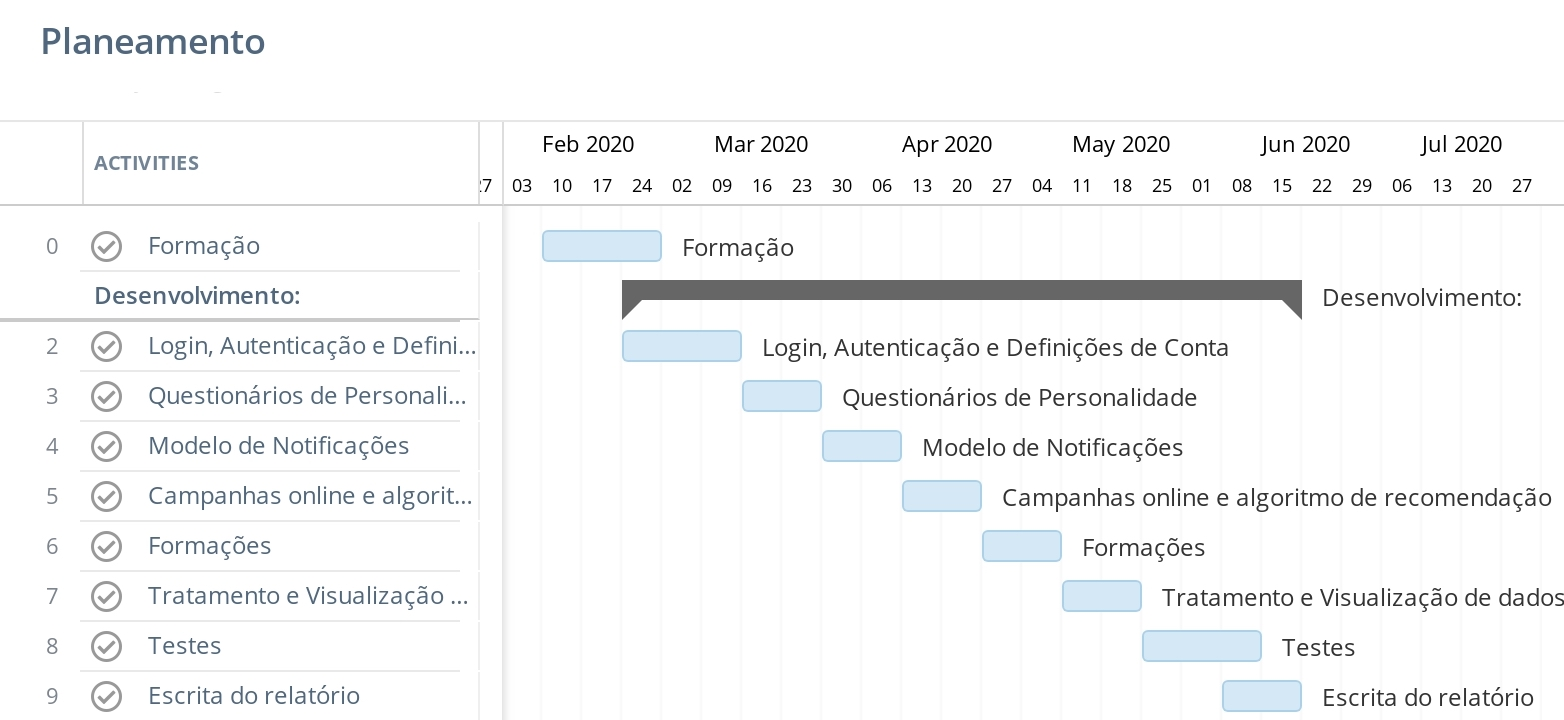
\includegraphics[width=1\textwidth]{img/gantt/semestre2.jpeg}
		\caption{Diagrama de Gantt - Planeamento do 2º semestre}
		\label{fig:gantt2}
	\end{center}
\end{figure}


\section{Análise de Riscos}
\label{analiseriscos}

Antes de se iniciar a fase de desenvolvimento do projeto é importante realizar uma análise aos possíveis riscos associados ao projeto. Desta forma é importante antecipar/identificar os diferentes riscos que contribuem para o insucesso do projeto para que se possam criar estratégias de mitigação de maneira a minimizar o impacto de cada risco. Os diferentes riscos serão classificados tendo em conta o seu impacto e a sua probabilidade.

\begin{itemize}
	\item[--] \textbf{Probabilidade}
	\subitem \textbf{Baixa}: Menor que 30\%
	\subitem \textbf{Média}: Entre 30\% a 70\%
	\subitem \textbf{Alta}: Superior a 70\%
	\item[--] \textbf{Impacto}
	\subitem \textbf{Baixo}: Interfere no desenvolvimento do projeto.
	\subitem \textbf{Médio}: Interfere no desenvolvimento do projeto e força alterações no produto final.
	\subitem \textbf{Alto}: Compromete a finalização do projeto.
\end{itemize}

De seguida serão listados todos os riscos associados ao projeto e respetivo plano de mitigação para tentar reduzir o impacto do mesmo:

\textbf{R01 - Dependência de sistemas externos}
\begin{itemize}
	\item[--] \textbf{ID}: R01
	\item[--] \textbf{Descrição}: Não se pode garantir uma disponibilidade de 100\% em todos os sistemas externos (e. g. APIs offline) sendo que em algumas ocasiões o sistema pode ter algumas funcionalidades indisponíveis.
	\item[--] \textbf{Estratégia de Mitigação}: Quando um serviço externo está temporariamente indisponível, apesar de algumas das respectivas funcionalidades também estarem indisponíveis, o sistema deve tratar os pedidos do utilizador de forma a não afetar a experiência do utilizador, ou no pior dos casos para reduzir o impacto no mesmo.
	\item[--] \textbf{Probabilidade}: Baixa
	\item[--] \textbf{Impacto}: Baixo
\end{itemize}

\textbf{R02 - Dificuldade em implementar o sistema de pagamento}
\begin{itemize}
	\item[--] \textbf{ID}: R02
	\item[--] \textbf{Descrição}: A falta de experiência por parte do aluno na implementação de métodos ou serviços de pagamentos põe em causa a boa implementação do mesmo e pode comprometer uma das principais funcionalidades do produto final.
	\item[--] \textbf{Estratégia de Mitigação}: Deve ser feita uma análise cuidada dos métodos ou serviços de pagamentos disponíveis para integrar com a tecnologia de desenvolvimento da plataforma e de seguida deve ser lida a documentação com atenção para garantir uma boa implementação da mesma.
	\item[--] \textbf{Probabilidade}: Alta
	\item[--] \textbf{Impacto}: Alto
\end{itemize}

\textbf{R03 - Adaptação a novas tecnologias }
\begin{itemize}
	\item[--] \textbf{ID}: R03
	\item[--] \textbf{Descrição}: A não familiarização, por parte do aluno, com as principais tecnologias que irão ser utilizadas na desenvolvimento do projeto, pode criar atrasos na implementação devido à falta de experiência e/ou subestimação do tempo definido para cada tarefa, comprometendo a implementação de algumas funcionalidades.
	\item[--] \textbf{Estratégia de Mitigação}: Para além das horas definidas no planeamento do projeto, o aluno terá de dispensar horas extra de modo a conseguir concluir a implementação e validação de todas as funcionalidades.
	\item[--] \textbf{Probabilidade}: Média
	\item[--] \textbf{Impacto}: Médio
\end{itemize}

\textbf{R04 - Novo requisito funcional}
\begin{itemize}
	\item[--] \textbf{ID}: R04
	\item[--] \textbf{Descrição}: As necessidades do cliente podem mudar com o tempo e nesse sentido é possível o aparecimento de um novo requisito funcional.
	\item[--] \textbf{Estratégia de Mitigação}: Reavaliação do plano de desenvolvimento e reestruturação de algumas funcionalidades, para que fiquem mais genéricas e assim, possa haver tempo para a realização do(s) novo(s) requisito(s). Em alternativa, poderão também ter que ser dispensadas algumas horas pelo aluno, de modo a cumprir com o plano de desenvolvimento.
	\item[--] \textbf{Probabilidade}: Baixa 
	\item[--] \textbf{Impacto}: Médio
\end{itemize}

\textbf{R05 - Falta de investimento no projeto}
\begin{itemize}
	\item[--] \textbf{ID}: R05
	\item[--] \textbf{Descrição}: As necessidades do cliente podem mudar com o tempo e haver uma mudança negativa na alocação de recursos ao projeto.
	\item[--] \textbf{Estratégia de Mitigação}: Para além das horas definidas no planeamento do projeto, o aluno terá de dispensar horas extra de modo a conseguir concluir a implementação e validação de todas as funcionalidades.
	\item[--] \textbf{Probabilidade}: Baixa 
	\item[--] \textbf{Impacto}: Alto
\end{itemize}

\textbf{R06 - \textit{Wishfull Thinking}}
\begin{itemize}
	\item[--] \textbf{ID}: R06
	\item[--] \textbf{Descrição}: Apesar da experiência por parte do cliente (i. e. 10.digital) no sector de marketing digital e na adopção de estratégias de inbound marketing, há sempre o risco do projeto ser apenas um \textit{wishfull thinking} e não ter o impacto esperado.
	\item[--] \textbf{Estratégia de Mitigação}: Devem ser feitos testes de usabilidade, seguidos de testes com utilizadores reais.
	\item[--] \textbf{Probabilidade}: Baixa
	\item[--] \textbf{Impacto}: Alto
\end{itemize}

Para uma melhor compreensão e visualização dos riscos associados ao projeto, apresenta-se na Tabela \ref{tab:riscos}, um resumo da probabilidade e o impacto de cada risco.

\begin{table}[ht!]
	\centering
	\begin{tabular}{ | l | l | l | l |}
		\hline
		\diagbox[width=15em]{Impacto}{Probabilidade}
		& Baixo & Médio & Alto\\
		\hline
		Baixa & \cellcolor{green}\centering R01 & \cellcolor{yellow}R04& \cellcolor{orange}\\
		\hline
		Média & \cellcolor{yellow} & \cellcolor{orange}R03 & \cellcolor{darkOrange}\\
		\hline
		Alta & \cellcolor{orange}R05 e R06 & \cellcolor{darkOrange} & \cellcolor{red}R02\\
		\hline
	\end{tabular}
	\begin{center}
		\caption {Classificação dos riscos associados ao projeto}
		\label {tab:riscos}
	\end{center}
\end{table}





\glsresetall



